% ============================================================================
% Lecture 22 (B21): Deep Surrogate Models
% Deep Learning for Solving and Estimating Dynamic Models in Economics and Finance
% Course author: Simon Scheidegger
% ============================================================================

\documentclass[aspectratio=169,11pt]{beamer}

% ---------- Theme and colors ----------
\usecolortheme{dove}
\setbeamertemplate{navigation symbols}{}
\setbeamertemplate{footline}{%
  \hfill\usebeamerfont{page number in head/foot}%
  \usebeamercolor[fg]{normal text}%
  \insertframenumber\,/\,\inserttotalframenumber\kern1em\vskip4pt}
\setbeamerfont{frametitle}{size=\huge}

% ---------- Packages ----------
\usepackage[utf8]{inputenc}
\usepackage[T1]{fontenc}
\usepackage{amsmath,amssymb,amsfonts}
\usepackage{bm}
\usepackage{graphicx}
\usepackage{tikz}
\usetikzlibrary{shapes,arrows.meta,positioning,calc,fit,backgrounds,patterns,decorations.pathreplacing}
\usepackage{pgfplots}
\pgfplotsset{compat=1.18}
\usepackage{booktabs}
\usepackage{hyperref}
\usepackage{multicol}
\usepackage{xcolor}
\usepackage{algorithm}
\usepackage{algorithmic}
\usepackage{listings}
\usepackage{pifont}

% ---------- Listings style for Python ----------
\lstset{
    language=Python,
    basicstyle=\small\ttfamily,
    keywordstyle=\color{uzhblue}\bfseries,
    commentstyle=\color{uzhgreydark}\itshape,
    stringstyle=\color{darkgreen},
    showstringspaces=false,
    breaklines=true,
    frame=none,
    xleftmargin=0pt,
    aboveskip=4pt,
    belowskip=4pt,
    escapeinside={(*@}{@*)},
}

% ---------- Custom colors ----------
\definecolor{uzhblue}{rgb}{0,0,0.5}
\definecolor{uzhgreylight}{RGB}{236,238,241}
\definecolor{uzhgreydark}{RGB}{81,86,94}
\definecolor{harvardcrimson}{RGB}{153,0,0}
\definecolor{unil@blue}{RGB}{0,140,204}
\definecolor{unil@black}{RGB}{35,31,32}
\definecolor{darkgreen}{RGB}{0,100,0}
\definecolor{darkred}{RGB}{139,0,0}
\definecolor{softblue}{RGB}{70,130,180}
\definecolor{softorange}{RGB}{230,159,0}
\definecolor{softgreen}{RGB}{0,158,115}

% ---------- Set beamer colors ----------
\setbeamercolor{frametitle}{bg=uzhgreylight, fg=uzhblue}
\setbeamercolor{title}{fg=uzhblue}
\setbeamercolor{structure}{fg=uzhblue}
\setbeamercolor{block title}{bg=unil@blue, fg=white}
\setbeamercolor{block body}{bg=uzhgreylight}
\setbeamercolor{block title alerted}{bg=darkred,fg=white}
\setbeamercolor{block body alerted}{bg=red!5}
\setbeamercolor{block title example}{bg=darkgreen,fg=white}
\setbeamercolor{block body example}{bg=green!5}
\setbeamercolor{item}{fg=unil@black}
\setbeamercolor{normal text}{fg=unil@black}

% ---------- Emphasis and hyperlinks ----------
\newcommand{\emphc}[1]{\textcolor{harvardcrimson}{#1}}
\hypersetup{colorlinks,linkcolor=harvardcrimson,urlcolor=harvardcrimson}

% ---------- Math commands ----------
\newcommand{\x}{\bm{x}}
\newcommand{\w}{\bm{w}}
\newcommand{\bb}{\bm{b}}
\newcommand{\z}{\bm{z}}
\newcommand{\W}{\bm{W}}
\newcommand{\X}{\bm{X}}
\renewcommand{\a}{\bm{a}}
\newcommand{\R}{\mathbb{R}}
\newcommand{\E}[1]{\mathbb{E}\!\left[#1\right]}
\DeclareMathOperator*{\argmin}{arg\,min}
\DeclareMathOperator*{\argmax}{arg\,max}

% ---------- Title ----------
\title[Lecture 23 (B22)]{Lecture 23 (B22): Gaussian Process Regression}
\subtitle{Kernels, posterior, hyperparameter learning, deep kernel learning}
\author{Simon Scheidegger}
\institute{HEC, University of Lausanne}
\date{}
\begin{document}

% Custom command used in some "Finger Exercise" frame titles.
\providecommand{\exercisepause}{%
  \tikz[baseline=(X.base)]{\node[fill=darkgreen!80!black, text=white,
  rounded corners=2pt, inner sep=3pt, font=\scriptsize\bfseries](X){PAUSE};}}

{\setbeamercolor{background canvas}{bg=uzhgreylight}
\begin{frame}
\titlepage
\end{frame}
}

\section{Gaussian Process Regression}

% --- Slide 16: Why Gaussian Processes? ---
\begin{frame}{Why Gaussian Processes?}
\begin{itemize}
  \item \textbf{Nonparametric:} No fixed architecture; the model grows with data.
  \item \textbf{Built-in uncertainty quantification:} Posterior mean \emph{and} variance at every point.
  \item \textbf{Principled kernel selection:} Encode prior beliefs about smoothness, periodicity, etc.
  \item \textbf{Hyperparameter learning:} Marginal likelihood provides a principled objective.
\end{itemize}

\vspace{0.3cm}
\begin{alertblock}{Complementary to DNNs}
\begin{itemize}
  \item GPs: best for moderate dimensions ($d \leq 10$) with built-in UQ.
  \item DNNs: best for high dimensions ($d \gg 10$) with large data.
  \item Combining both is a powerful strategy (cf.\ slide~9).
\end{itemize}
\end{alertblock}

\vspace{0.15cm}
{\tiny \textbf{Foundations:} Rasmussen \& Williams (2006); MacKay (1992); Krause, Singh \& Guestrin (2008).
\textbf{In DP:} Engel, Mannor \& Meir (2005); Deisenroth, Rasmussen \& Peters (2009).
\textbf{Sparse / scalable:} Titsias (2009); Hensman, Fusi \& Lawrence (2013).}
\end{frame}

% --- Foundational slides (from Bundesbank version) ---
\begin{frame}{Recall: Multivariate Gaussians}
\begin{columns}[T]
\begin{column}{0.45\textwidth}
A random vector $\bm{x} \in \R^d$ is \emphc{multivariate Gaussian} if
\[
\bm{x} \sim \mathcal{N}(\bm{\mu}, \Sigma)
\]
with density
{\small
\[
p(\bm{x}) \propto
\exp\!\Bigl(-\tfrac{1}{2}(\bm{x}\!-\!\bm{\mu})^\top \Sigma^{-1}(\bm{x}\!-\!\bm{\mu})\Bigr)
\]
}

\vspace{0.2cm}
\begin{block}{Key fact}
A multivariate Gaussian is \emphc{fully characterized} by its mean vector $\bm{\mu}$ and covariance matrix $\Sigma$.
\end{block}
\end{column}

\begin{column}{0.52\textwidth}
\begin{center}
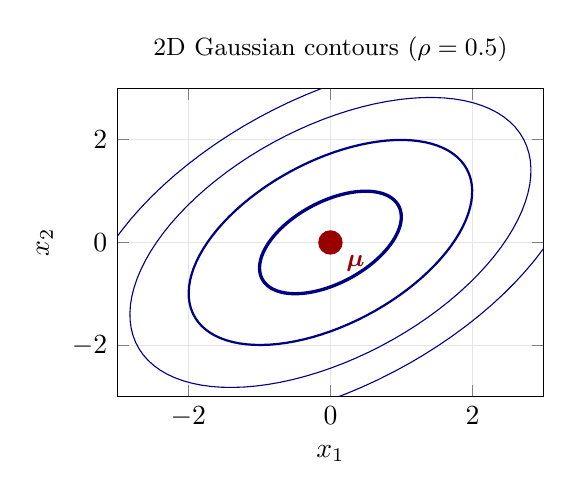
\begin{tikzpicture}
\begin{axis}[
    width=7cm, height=5.5cm,
    xlabel={$x_1$}, ylabel={$x_2$},
    xmin=-3, xmax=3, ymin=-3, ymax=3,
    grid=major, grid style={gray!20},
    every axis plot/.append style={no markers},
    title={\small 2D Gaussian contours ($\rho=0.5$)},
]
\addplot[uzhblue, very thick, domain=0:360, samples=100]
    ({0.707*(1.22*cos(x) - 0.707*sin(x))}, {0.707*(1.22*cos(x) + 0.707*sin(x))});
\addplot[uzhblue, thick, domain=0:360, samples=100]
    ({1.414*(1.22*cos(x) - 0.707*sin(x))}, {1.414*(1.22*cos(x) + 0.707*sin(x))});
\addplot[uzhblue, domain=0:360, samples=100]
    ({2.0*(1.22*cos(x) - 0.707*sin(x))}, {2.0*(1.22*cos(x) + 0.707*sin(x))});
\addplot[uzhblue, thin, domain=0:360, samples=100]
    ({2.5*(1.22*cos(x) - 0.707*sin(x))}, {2.5*(1.22*cos(x) + 0.707*sin(x))});
\addplot[only marks, mark=+, mark size=4pt, harvardcrimson, thick] coordinates {(0,0)};
\node[font=\small, harvardcrimson] at (axis cs:0.35,-0.4) {$\bm{\mu}$};
\end{axis}
\end{tikzpicture}
\end{center}
\end{column}
\end{columns}
\end{frame}

\begin{frame}{Joint and Conditional Distributions}
\begin{columns}[T]
\begin{column}{0.48\textwidth}
\textbf{Joint distribution:}
\[
\begin{pmatrix} x_1 \\ x_2 \end{pmatrix}
\sim \mathcal{N}\!\left(
\begin{pmatrix} \mu_1 \\ \mu_2 \end{pmatrix},
\begin{pmatrix} \Sigma_{11} & \Sigma_{12} \\ \Sigma_{21} & \Sigma_{22} \end{pmatrix}
\right)
\]

\vspace{0.3cm}
\textbf{Conditional distribution:}
\begin{align*}
\mu_{1|2} &= \mu_1 + \Sigma_{12}\Sigma_{22}^{-1}(x_2 - \mu_2)\\
\Sigma_{1|2} &= \Sigma_{11} - \Sigma_{12}\Sigma_{22}^{-1}\Sigma_{21}
\end{align*}

\vspace{0.1cm}
\emphc{This is the mathematical engine behind GP regression.}
\end{column}

\begin{column}{0.50\textwidth}
\begin{center}
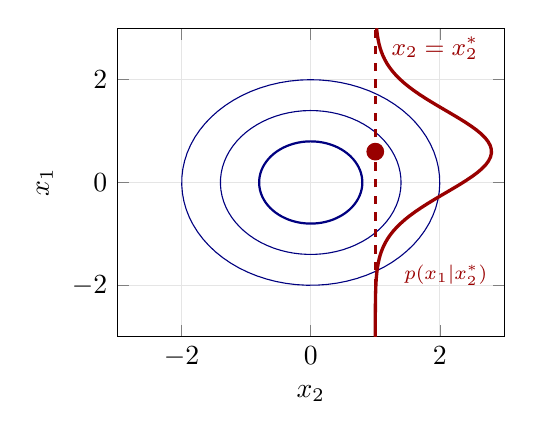
\begin{tikzpicture}
\begin{axis}[
    width=6.5cm, height=5.5cm,
    xlabel={$x_2$}, ylabel={$x_1$},
    xmin=-3, xmax=3, ymin=-3, ymax=3,
    grid=major, grid style={gray!20},
    every axis plot/.append style={no markers},
]
\addplot[uzhblue, thick, domain=0:360, samples=80]
    ({0.8*(0.894*cos(x) - 0.447*sin(x))}, {0.8*(0.447*cos(x) + 0.894*sin(x))});
\addplot[uzhblue, domain=0:360, samples=80]
    ({1.4*(0.894*cos(x) - 0.447*sin(x))}, {1.4*(0.447*cos(x) + 0.894*sin(x))});
\addplot[uzhblue, thin, domain=0:360, samples=80]
    ({2.0*(0.894*cos(x) - 0.447*sin(x))}, {2.0*(0.447*cos(x) + 0.894*sin(x))});
\draw[harvardcrimson, very thick, dashed] (axis cs:1,-3) -- (axis cs:1,3);
\node[font=\small, harvardcrimson, anchor=south west] at (axis cs:1.1,2.2) {$x_2 = x_2^*$};
\addplot[harvardcrimson, very thick, domain=-3:3, samples=80]
    ({1 + 1.8*exp(-(x-0.6)^2/(2*0.64))}, {x});
\node[font=\scriptsize, harvardcrimson, anchor=west, inner sep=1pt]
    at (axis cs:1.4,-1.8) {$p(x_1|x_2^*)$};
\addplot[only marks, mark=*, mark size=3pt, harvardcrimson] coordinates {(1,0.6)};
\end{axis}
\end{tikzpicture}
\end{center}
{\small ``Slicing'' the joint at $x_2 = x_2^*$ yields a 1D Gaussian.}
\end{column}
\end{columns}
\end{frame}

\begin{frame}{From Observations to Interpolation}
\vspace{-0.2cm}
\begin{columns}[T]
\begin{column}{0.38\textwidth}
\begin{center}
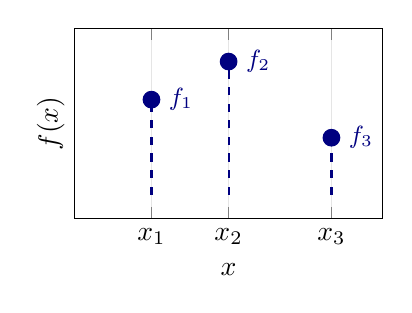
\begin{tikzpicture}
\begin{axis}[
    width=5.5cm, height=4cm,
    xlabel={$x$}, ylabel={$f(x)$},
    xmin=-0.5, xmax=5.5, ymin=-0.5, ymax=3.5,
    grid=major, grid style={gray!20},
    xtick={1,2.5,4.5},
    xticklabels={$x_1$,$x_2$,$x_3$},
    ytick=\empty,
    every axis plot/.append style={no markers},
]
\addplot[uzhblue, thick, dashed] coordinates {(1,0) (1,2.0)};
\addplot[uzhblue, thick, dashed] coordinates {(2.5,0) (2.5,2.8)};
\addplot[uzhblue, thick, dashed] coordinates {(4.5,0) (4.5,1.2)};
\addplot[only marks, mark=*, mark size=3pt, uzhblue] coordinates
    {(1,2.0) (2.5,2.8) (4.5,1.2)};
\node[font=\small, uzhblue, anchor=west] at (axis cs:1.15,2.0) {$f_1$};
\node[font=\small, uzhblue, anchor=west] at (axis cs:2.65,2.8) {$f_2$};
\node[font=\small, uzhblue, anchor=west] at (axis cs:4.65,1.2) {$f_3$};
\end{axis}
\end{tikzpicture}
\end{center}
\end{column}

\begin{column}{0.60\textwidth}
\textbf{Assume} function values are jointly Gaussian:
\vspace{-0.2cm}
{\small
\[
\begin{pmatrix} f_1 \\ f_2 \\ f_3 \end{pmatrix}
\sim \mathcal{N}\!\left(
\bm{0},\;
\begin{pmatrix} K_{11} & K_{12} & K_{13} \\ K_{21} & K_{22} & K_{23} \\ K_{31} & K_{32} & K_{33} \end{pmatrix}
\right)
\]
}

\vspace{-0.1cm}
\emphc{Nearby points ($f_1, f_2$) should be more correlated than distant ones ($f_1, f_3$).}

\vspace{0.1cm}
\textbf{Example:}\;
$K = \bigl(\begin{smallmatrix} 1.0 & 0.7 & 0.2 \\ 0.7 & 1.0 & 0.6 \\ 0.2 & 0.6 & 1.0 \end{smallmatrix}\bigr)$

\vspace{0.15cm}
Covariance via a \emphc{kernel function}: $K_{ij} = k(x_i, x_j)$

\vspace{0.1cm}
{\small $\Rightarrow$ The kernel encodes our prior belief about function smoothness.}
\end{column}
\end{columns}
\end{frame}

% --- GP — A Distribution Over Functions ---
\begin{frame}{GP: A Distribution Over Functions}
\begin{block}{Definition}
A \emphc{Gaussian Process} is a collection of random variables, any finite number of which have a joint Gaussian distribution:
\[
f(\x) \sim \mathcal{GP}\bigl(\mu(\x),\; k(\x, \x')\bigr).
\]
\end{block}

\begin{itemize}
  \item \textbf{Mean function:} $\mu(\x) = \E{f(\x)}$ \quad (often set to $0$).
  \item \textbf{Covariance function (kernel):} $k(\x,\x') = \E{(f(\x)-\mu(\x))(f(\x')-\mu(\x'))^\top}$.
\end{itemize}

\vspace{0.3cm}
\begin{center}
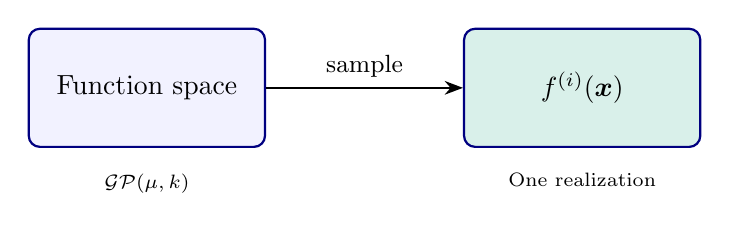
\begin{tikzpicture}[>=Stealth]
\node[draw=uzhblue, thick, rounded corners, fill=blue!5,
      minimum width=3cm, minimum height=1.5cm] (fspace) {Function space};
\node[right=2.5cm of fspace, draw=uzhblue, thick, rounded corners, fill=softgreen!15,
      minimum width=3cm, minimum height=1.5cm] (sample) {$f^{(i)}(\x)$};
\draw[->, thick] (fspace) -- node[above, font=\small]{sample} (sample);
\node[below=0.2cm of fspace, font=\scriptsize] {$\mathcal{GP}(\mu, k)$};
\node[below=0.2cm of sample, font=\scriptsize] {One realization};
\end{tikzpicture}
\end{center}
\end{frame}

% --- Slide 18: The Squared Exponential Kernel ---
\begin{frame}{The Squared Exponential (RBF) Kernel}
\[
k_{SE}(x, x') = \sigma_f^2 \exp\!\left(-\frac{(x - x')^2}{2\ell^2}\right)
\]

\begin{itemize}
  \item $\ell$ = \textbf{length scale} (horizontal correlation range)
  \item $\sigma_f^2$ = \textbf{signal variance} (vertical scale)
\end{itemize}

\vspace{0.2cm}
\begin{center}
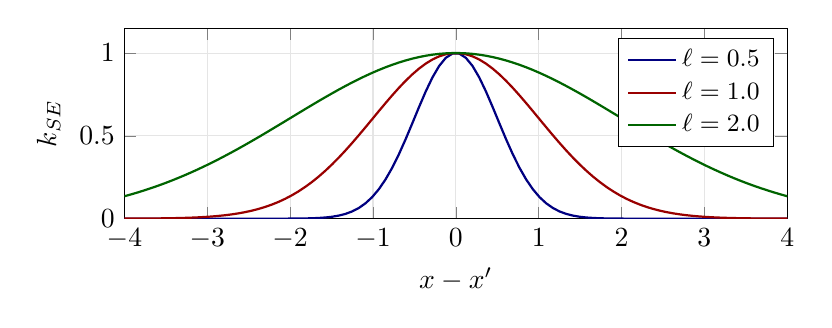
\begin{tikzpicture}
\begin{axis}[
    width=10cm, height=4cm,
    xlabel={$x - x'$}, ylabel={$k_{SE}$},
    xmin=-4, xmax=4, ymin=0, ymax=1.15,
    legend style={at={(0.98,0.95)}, anchor=north east, font=\small},
    grid=major, grid style={gray!20},
    every axis plot/.append style={thick, no markers},
]
\addplot[uzhblue, domain=-4:4, samples=100] {exp(-x^2/(2*0.5^2))};
\addlegendentry{$\ell=0.5$}
\addplot[harvardcrimson, domain=-4:4, samples=100] {exp(-x^2/(2*1.0^2))};
\addlegendentry{$\ell=1.0$}
\addplot[darkgreen, domain=-4:4, samples=100] {exp(-x^2/(2*2.0^2))};
\addlegendentry{$\ell=2.0$}
\end{axis}
\end{tikzpicture}
\end{center}

{\small Larger $\ell$ $\Rightarrow$ smoother functions; smaller $\ell$ $\Rightarrow$ more wiggly.}
\end{frame}

% --- Kernel slides (from Bundesbank version) ---
\begin{frame}{The Mat\'ern Kernel Family}
\vspace{-0.2cm}
{\small
$k_{\text{Mat}}(r) = \sigma^2 \frac{2^{1-\nu}}{\Gamma(\nu)}
\bigl(\frac{\sqrt{2\nu}\,r}{\ell}\bigr)^{\!\nu}
K_\nu\!\bigl(\frac{\sqrt{2\nu}\,r}{\ell}\bigr),
\quad r = |x - x'|$}

\vspace{-0.2cm}
\begin{center}
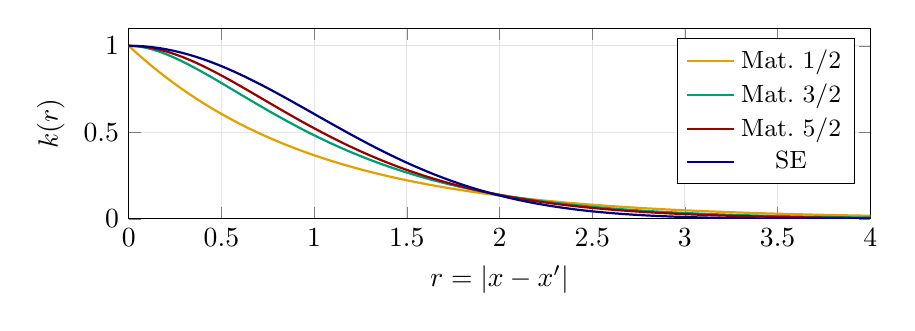
\begin{tikzpicture}
\begin{axis}[
    width=11cm, height=4cm,
    xlabel={$r = |x - x'|$}, ylabel={$k(r)$},
    xmin=0, xmax=4, ymin=0, ymax=1.1,
    grid=major, grid style={gray!20},
    every axis plot/.append style={thick, no markers},
    legend style={at={(0.98,0.95)}, anchor=north east, font=\small},
]
\addplot[softorange, domain=0:4, samples=100] {exp(-x)};
\addlegendentry{Mat.\ 1/2}
\addplot[softgreen, domain=0:4, samples=100] {(1+1.732*x)*exp(-1.732*x)};
\addlegendentry{Mat.\ 3/2}
\addplot[harvardcrimson, domain=0:4, samples=100] {(1+2.236*x+5/3*x^2)*exp(-2.236*x)};
\addlegendentry{Mat.\ 5/2}
\addplot[uzhblue, domain=0:4, samples=100] {exp(-x^2/2)};
\addlegendentry{SE}
\end{axis}
\end{tikzpicture}
\end{center}

\vspace{-0.2cm}
{\small
\begin{itemize}\setlength{\itemsep}{0pt}
  \item $\nu$ controls \emphc{smoothness}: $\nu\!=\!3/2$ $\Rightarrow$ once differentiable;\; $\nu\!=\!5/2$ $\Rightarrow$ twice;\; SE $\Rightarrow$ $\infty$-smooth.
  \item \textbf{Use case:} Mat\'ern when the true function is \emph{not} infinitely smooth (e.g., has kinks).
\end{itemize}}
\end{frame}

\begin{frame}[shrink=5]{Combining Kernels}
Kernels can be \emphc{added} and \emphc{multiplied} to compose complex priors from simple blocks.

\vspace{0.3cm}
\begin{columns}[T]
\column{0.55\textwidth}
\begin{center}
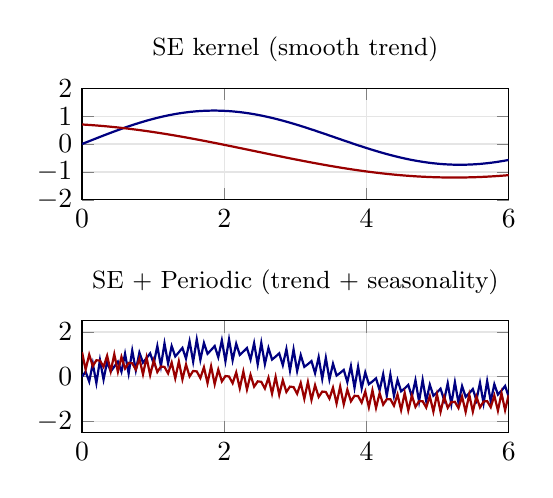
\begin{tikzpicture}
\begin{axis}[
    name=kse,
    width=7cm, height=3cm,
    title={\small SE kernel (smooth trend)},
    xmin=0, xmax=6, ymin=-2, ymax=2,
    grid=major, grid style={gray!20},
    every axis plot/.append style={thick, no markers},
]
\addplot[uzhblue, domain=0:6, samples=80] {sin(deg(0.9*x)) + 0.3*sin(deg(0.4*x))};
\addplot[harvardcrimson, domain=0:6, samples=80] {0.7*cos(deg(0.6*x)) - 0.5*sin(deg(0.3*x))};
\end{axis}

\begin{axis}[
    at={(kse.below south)}, anchor=above north, yshift=-0.3cm,
    width=7cm, height=3cm,
    title={\small SE $+$ Periodic (trend + seasonality)},
    xmin=0, xmax=6, ymin=-2.5, ymax=2.5,
    grid=major, grid style={gray!20},
    every axis plot/.append style={thick, no markers},
]
\addplot[uzhblue, domain=0:6, samples=120]
    {sin(deg(0.9*x)) + 0.3*sin(deg(0.4*x)) + 0.5*sin(deg(180*x))};
\addplot[harvardcrimson, domain=0:6, samples=120]
    {0.7*cos(deg(0.6*x)) - 0.5*sin(deg(0.3*x)) + 0.4*cos(deg(180*x))};
\end{axis}
\end{tikzpicture}
\end{center}

\column{0.42\textwidth}
\begin{block}{Kernel algebra}
\begin{itemize}\setlength{\itemsep}{3pt}
  \item \textbf{$k_1 + k_2$} (OR):\\
  high if \emph{either} is high\\
  $\Rightarrow$ trend + seasonality
  \item \textbf{$k_1 \times k_2$} (AND):\\
  high only if \emph{both} high\\
  $\Rightarrow$ locally periodic
\end{itemize}
\end{block}

\vspace{0.3cm}
{\small \emphc{Compose complex priors} from simple building blocks.}
\end{columns}
\end{frame}

% --- Sampling from the GP Prior ---
\begin{frame}{Sampling from the GP Prior}
\begin{columns}[T]
\begin{column}{0.42\textwidth}
\begin{block}{Algorithm}
\begin{enumerate}\setlength{\itemsep}{1pt}
  \item Grid $x_{1:N}$ over domain
  \item $K_{ij} = k(x_i, x_j)$
  \item Cholesky: $K = LL^\top$
  \item $\bm{f}^{(s)} = L \cdot \bm{u}$, $\bm{u} \sim \mathcal{N}(\bm{0}, I)$
\end{enumerate}
\end{block}
\vspace{0.2cm}
{\small Five functions drawn from a GP prior with SE kernel ($\ell=1$, $\sigma_f=1$).}
\end{column}
\begin{column}{0.56\textwidth}
\begin{center}
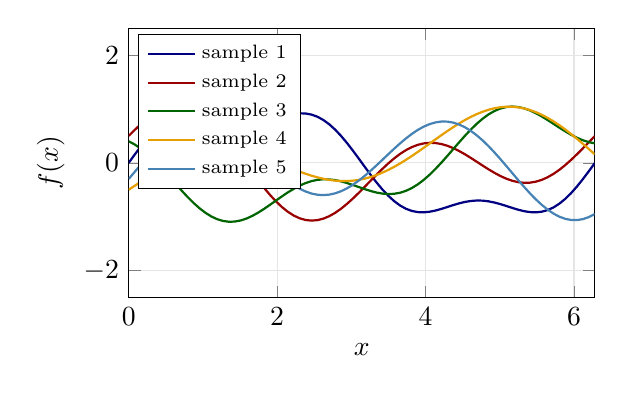
\begin{tikzpicture}
\begin{axis}[
    width=7.5cm, height=5cm,
    xlabel={$x$}, ylabel={$f(x)$},
    xmin=0, xmax=6.28, ymin=-2.5, ymax=2.5,
    grid=major, grid style={gray!20},
    every axis plot/.append style={thick, no markers},
    legend style={at={(0.02,0.98)}, anchor=north west, font=\scriptsize},
]
\addplot[uzhblue, domain=0:6.28, samples=80] {sin(deg(x)) + 0.3*sin(deg(3*x))};
\addlegendentry{sample 1}
\addplot[harvardcrimson, domain=0:6.28, samples=80] {0.5*cos(deg(x)) + 0.7*sin(deg(2*x))};
\addlegendentry{sample 2}
\addplot[darkgreen, domain=0:6.28, samples=80] {-0.8*sin(deg(0.8*x)) + 0.4*cos(deg(2.5*x))};
\addlegendentry{sample 3}
\addplot[softorange, domain=0:6.28, samples=80] {0.6*sin(deg(1.5*x)) - 0.5*cos(deg(0.7*x))};
\addlegendentry{sample 4}
\addplot[softblue, domain=0:6.28, samples=80] {-0.3*cos(deg(1.2*x)) + 0.9*sin(deg(1.8*x))};
\addlegendentry{sample 5}
\end{axis}
\end{tikzpicture}
\end{center}
\end{column}
\end{columns}
\end{frame}

% --- Slide 20: From Prior to Posterior ---
\begin{frame}{From Prior to Posterior: Bayes Rule}
\begin{itemize}
  \item \textbf{Training set:} $\mathcal{D} = \{(\x_i, y_i)\}_{i=1}^n$.
  \item \textbf{Test points:} $\X_*$ where we want predictions.
  \item Joint distribution of training outputs $\bm{f}$ and test outputs $\bm{f}_*$ is Gaussian.
\end{itemize}

\vspace{0.3cm}
\begin{center}
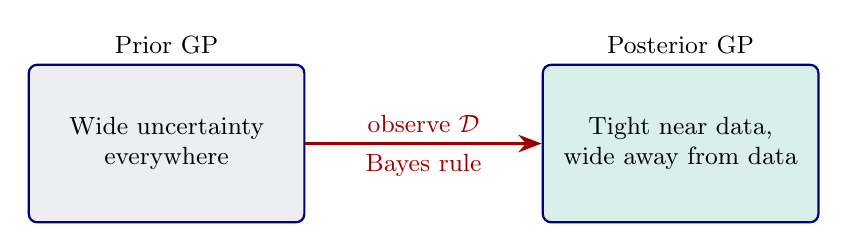
\begin{tikzpicture}[
    mlstep/.style={rectangle, draw=uzhblue, fill=uzhgreylight,
        minimum width=3.5cm, minimum height=2cm, rounded corners=3pt, thick},
    >=Stealth
]
\node[mlstep, label={[font=\small]above:Prior GP}] (prior) {
    \begin{minipage}{3cm}\centering
    \small Wide uncertainty\\everywhere
    \end{minipage}};
\node[mlstep, right=3cm of prior, fill=softgreen!15,
      label={[font=\small]above:Posterior GP}] (post) {
    \begin{minipage}{3cm}\centering
    \small Tight near data,\\wide away from data
    \end{minipage}};
\draw[->, very thick, harvardcrimson] (prior) -- node[above, font=\small]{observe $\mathcal{D}$}
    node[below, font=\small]{\emphc{Bayes rule}} (post);
\end{tikzpicture}
\end{center}

\vspace{0.2cm}
The posterior is \emph{still a GP} --- fully characterized by updated mean and covariance.
\end{frame}

% --- Slide 21: Noiseless GP Regression ---
\begin{frame}{Noiseless GP Regression}
\textbf{Joint distribution:}
\[
\begin{pmatrix} \bm{f} \\ \bm{f}_* \end{pmatrix}
\sim \mathcal{N}\!\left(
\begin{pmatrix} \bm{\mu} \\ \bm{\mu}_* \end{pmatrix},
\begin{pmatrix} K & K_* \\ K_*^\top & K_{**} \end{pmatrix}
\right)
\]

where $K_{ij} = k(\x_i, \x_j)$, \; $(K_*)_{ij} = k(\x_i, \x_*^{(j)})$, \; $(K_{**})_{ij} = k(\x_*^{(i)}, \x_*^{(j)})$.

\vspace{0.3cm}
\textbf{Posterior} (conditioning on $\bm{f}$):
\begin{align}
\bm{\mu}_{*|\mathcal{D}} &= K_*^\top K^{-1}(\bm{f} - \bm{\mu}) + \bm{\mu}_* \label{eq:gp_mean}\\
\Sigma_{*|\mathcal{D}} &= K_{**} - K_*^\top K^{-1} K_* \label{eq:gp_var}
\end{align}

\vspace{0.2cm}
\begin{alertblock}{Key insight}
\begin{itemize}
  \item Near observed data: $K_*^\top K^{-1} K_* \approx K_{**}$ $\Rightarrow$ \emphc{small variance}.
  \item Far from data: $K_*^\top K^{-1} K_* \approx 0$ $\Rightarrow$ \emphc{large variance} (reverts to prior).
\end{itemize}
\end{alertblock}
\end{frame}

% --- Slide 22: Prediction at a Single Test Point ---
\begin{frame}{Prediction at a Single Test Point}
\small
\textbf{Noiseless setting} ($\sigma_y^2 \to 0$ limit; GP interpolates training data). For a single test input $\x_*$:
\vspace{-4pt}
\begin{align}
\bar{f}_* &= \bm{k}_*^\top K^{-1} \bm{f} = \sum_{i=1}^{N} \alpha_i \, k(\x_i, \x_*) \\
\sigma_*^2 &= k(\x_*, \x_*) - \bm{k}_*^\top K^{-1} \bm{k}_*
\end{align}
\vspace{-12pt}

where $\bm{\alpha} = K^{-1}\bm{f}$, $\bm{k}_* = (k(\x_1, \x_*), \dots, k(\x_N, \x_*))^\top$. Noisy form ($K \to K + \sigma_y^2 I$) on next slide.

\begin{block}{Interpretation}
Posterior mean is a \emphc{weighted sum of kernel basis functions} centered at training points:
\vspace{-4pt}
\[
\bar{f}_* = \sum_{i=1}^N \alpha_i \, k(\x_i, \x_*)
\]
\vspace{-10pt}

Each observation $\x_i$ ``pulls'' the prediction via its kernel similarity to $\x_*$.
\end{block}
\end{frame}

% --- Slide 23: GPR with Noisy Data ---
\begin{frame}{GP Regression with Noisy Observations}
\textbf{Observation model:}
\[
y = f(\x) + \varepsilon, \qquad \varepsilon \sim \mathcal{N}(0, \sigma_y^2)
\]

\vspace{0.2cm}
The covariance of \emph{observations} becomes:
\[
\text{cov}[y_p, y_q] = k(\x_p, \x_q) + \sigma_y^2 \delta_{pq}
\]

\vspace{0.2cm}
In matrix form: replace $K$ with
\[
K_y = K + \sigma_y^2 I
\]

\vspace{0.3cm}
\begin{block}{Effect of noise}
\begin{itemize}
  \item Predictions no longer interpolate the data exactly.
  \item Even at training points, there is \emphc{residual uncertainty}.
  \item The noise term $\sigma_y^2 I$ also acts as \emphc{numerical regularization} (``nugget'' / ``jitter'').
\end{itemize}
\end{block}
\end{frame}

% --- Slide 24: Noisy GPR Posterior ---
\begin{frame}{Noisy GPR: Posterior Equations}
\textbf{Posterior mean and variance with noise:}
\begin{align}
\bar{f}_* &= \bm{k}_*^\top (K + \sigma_y^2 I)^{-1} \bm{y} \\
\sigma_*^2 &= k(\x_*, \x_*) - \bm{k}_*^\top (K + \sigma_y^2 I)^{-1} \bm{k}_*
\end{align}

\vspace{0.3cm}
\begin{columns}[T]
\begin{column}{0.48\textwidth}
\textbf{Noiseless} ($\sigma_y^2 = 0$):
\begin{itemize}
  \item Interpolates training points exactly
  \item Variance = 0 at training inputs
  \item Requires $K$ to be positive definite
\end{itemize}
\end{column}
\begin{column}{0.48\textwidth}
\textbf{Noisy} ($\sigma_y^2 > 0$):
\begin{itemize}
  \item Smooths through training points
  \item Variance $> 0$ everywhere
  \item Better numerical conditioning
\end{itemize}
\end{column}
\end{columns}

\vspace{0.3cm}
{\small \textbf{In practice:} Even for noiseless surrogates, adding a small jitter $\sigma_y^2 \sim 10^{-6}$ improves numerical stability.}
\end{frame}

% --- Slide 25: Effect of Kernel Parameters ---
\begin{frame}{The Effect of Kernel Parameters}
\begin{center}
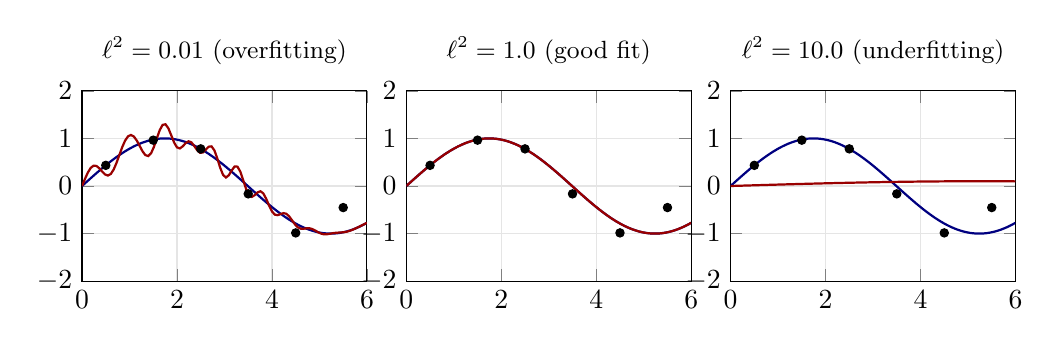
\begin{tikzpicture}
% Panel 1: small length scale (overfit)
\begin{axis}[
    name=plot1,
    width=5.2cm, height=4cm,
    title={\small $\ell^2 = 0.01$ (overfitting)},
    xmin=0, xmax=6, ymin=-2, ymax=2,
    grid=major, grid style={gray!20},
    every axis plot/.append style={no markers},
]
\addplot[uzhblue, thick, domain=0:6, samples=100] {sin(deg(0.9*x))};
\addplot[harvardcrimson, thick, domain=0:6, samples=100]
    {sin(deg(0.9*x)) + 0.3*sin(deg(8*x))*exp(-0.5*(x-1)^2) + 0.2*sin(deg(12*x))*exp(-0.5*(x-3)^2)};
\addplot[only marks, mark=*, mark size=1.5pt] coordinates
    {(0.5,0.434) (1.5,0.963) (2.5,0.780) (3.5,-0.165) (4.5,-0.985) (5.5,-0.453)};
\end{axis}

% Panel 2: good length scale
\begin{axis}[
    name=plot2, at={(plot1.east)}, anchor=west, xshift=0.5cm,
    width=5.2cm, height=4cm,
    title={\small $\ell^2 = 1.0$ (good fit)},
    xmin=0, xmax=6, ymin=-2, ymax=2,
    grid=major, grid style={gray!20},
    every axis plot/.append style={no markers},
]
\addplot[uzhblue, thick, domain=0:6, samples=100] {sin(deg(0.9*x))};
\addplot[harvardcrimson, thick, domain=0:6, samples=100] {sin(deg(0.9*x))};
\addplot[only marks, mark=*, mark size=1.5pt] coordinates
    {(0.5,0.434) (1.5,0.963) (2.5,0.780) (3.5,-0.165) (4.5,-0.985) (5.5,-0.453)};
\end{axis}

% Panel 3: large length scale (underfit)
\begin{axis}[
    name=plot3, at={(plot2.east)}, anchor=west, xshift=0.5cm,
    width=5.2cm, height=4cm,
    title={\small $\ell^2 = 10.0$ (underfitting)},
    xmin=0, xmax=6, ymin=-2, ymax=2,
    grid=major, grid style={gray!20},
    every axis plot/.append style={no markers},
]
\addplot[uzhblue, thick, domain=0:6, samples=100] {sin(deg(0.9*x))};
\addplot[harvardcrimson, thick, domain=0:6, samples=100] {0.1*sin(deg(0.3*x))};
\addplot[only marks, mark=*, mark size=1.5pt] coordinates
    {(0.5,0.434) (1.5,0.963) (2.5,0.780) (3.5,-0.165) (4.5,-0.985) (5.5,-0.453)};
\end{axis}
\end{tikzpicture}
\end{center}

\vspace{0.2cm}
\begin{itemize}
  \item \textcolor{uzhblue}{\textbf{Blue:}} true function $f(x) = \sin(0.9x)$.
  \item \textcolor{harvardcrimson}{\textbf{Red:}} GP posterior mean.
  \item \textbf{Too small $\ell$:} overfits noise/wiggles. \quad \textbf{Too large $\ell$:} underfits, misses structure.
\end{itemize}

$\Rightarrow$ We need a principled way to learn $\ell$ and $\sigma_f^2$.
\end{frame}

% --- Slide 26: Learning Hyperparameters ---
\begin{frame}{Learning Kernel Hyperparameters}
\textbf{Problem:} How to choose $\ell$, $\sigma_f$, $\sigma_y$?  $\Rightarrow$ Maximize the \emphc{marginal likelihood}.

\vspace{0.2cm}
\begin{block}{Marginal likelihood (model evidence)}
\[
\log p(\bm{y}\,|\,\X) = \underbrace{-\tfrac{1}{2}\bm{y}^\top K_y^{-1}\bm{y}}_{\text{data fit}}
\underbrace{-\tfrac{1}{2}\log|K_y|}_{\text{complexity penalty}}
\underbrace{-\tfrac{N}{2}\log(2\pi)}_{\text{constant}}
\]
\end{block}

\vspace{0.1cm}
\begin{columns}[T]
\begin{column}{0.48\textwidth}
\textbf{Intuition:}
\begin{itemize}\setlength{\itemsep}{2pt}
  \item \textbf{Data fit} $\uparrow$: reward explaining observations
  \item \textbf{Complexity} $\downarrow$: penalize overly flexible models
  \item Balance $=$ \emphc{automatic Occam's razor}
\end{itemize}
\end{column}
\begin{column}{0.48\textwidth}
\textbf{Optimization:}
\begin{itemize}\setlength{\itemsep}{2pt}
  \item Gradient ascent on $\log p(\bm{y}|\X)$
  \item Hyperparameters: $\theta = \{\ell, \sigma_f, \sigma_y\}$
  \item Closed-form gradients available
  \item Implemented in scikit-learn, GPyTorch
\end{itemize}
\end{column}
\end{columns}
\end{frame}

% --- New slide: Leave-one-out predictive error ---
\begin{frame}{Leave-One-Out Predictive Error}
\textbf{Idea.} Quantify out-of-sample predictive accuracy without holding out data.

\smallskip
For a GP with training set $\{(\x_i, y_i)\}_{i=1}^n$ and noise variance $\sigma_y^2$:
\begin{equation*}
\mu_{-i}(\x_i) - y_i \;=\; -\frac{[K_y^{-1}\bm y]_i}{[K_y^{-1}]_{ii}}, \qquad
\sigma_{-i}^2(\x_i) \;=\; \frac{1}{[K_y^{-1}]_{ii}}.
\end{equation*}

\smallskip
\textbf{Why it's free.}
\begin{itemize}\itemsep0pt
  \item $K_y^{-1}$ is recovered from the same Cholesky factor used for posterior inference
  \item LOO across all $n$ points: $\mathcal{O}(n^2)$ on top of the existing $\mathcal{O}(n^3)$
  \item No new training, no held-out split lost
\end{itemize}

\smallskip
\textbf{Use cases.} Surrogate-health diagnostic across iterations of GP-VFI (Part IV) and across active-learning rounds in SMM (companion exercise deck).

\medskip
{\scriptsize Closed form: Rasmussen \& Williams (2006), \S5.4.2.}
\end{frame}

% --- Slide 27: GPR Example Code ---
\begin{frame}[fragile]{GPR: Numpy Implementation Sketch}
\begin{lstlisting}[basicstyle=\footnotesize\ttfamily]
import numpy as np
from scipy.linalg import cho_factor, cho_solve

def kernel(X1, X2, l=1.0, sf=1.0):
    sq = np.sum(X1**2,1).reshape(-1,1) \
         + np.sum(X2**2,1) - 2*X1@X2.T
    return sf**2 * np.exp(-0.5 * sq / l**2)

K = kernel(X_tr, X_tr) + 1e-8*np.eye(N)
L, low = cho_factor(K, lower=True)  # Cholesky
alpha = cho_solve((L, low), y_tr)   # weights

Ks = kernel(X_tr, X_te)
mu  = Ks.T @ alpha                  # mean
v   = cho_solve((L, low), Ks)
var = kernel(X_te, X_te) - Ks.T @ v # variance
\end{lstlisting}

\vspace{0.2cm}
{\small See \textbf{Algorithm 2.1} in Rasmussen \& Williams (2006), and notebook \texttt{02\_GP\_and\_BAL.ipynb}.}
\end{frame}

% --- Slide 28: GP in Practice ---
\begin{frame}{GP in Practice: scikit-learn \& GPyTorch}
\begin{columns}[T]
\begin{column}{0.48\textwidth}
\textbf{scikit-learn:}
\begin{itemize}
  \item \texttt{GaussianProcessRegressor}
  \item Automatic hyperparameter tuning via marginal likelihood
  \item Great for prototyping ($N \leq 10^4$)
  \item CPU only
\end{itemize}
\end{column}
\begin{column}{0.48\textwidth}
\textbf{GPyTorch:}
\begin{itemize}
  \item GPU-accelerated GP inference
  \item Scalable to $N > 10^5$ (inducing points, KISS-GP)
  \item Integrates with PyTorch ecosystem
  \item Production-ready
\end{itemize}
\end{column}
\end{columns}

\vspace{0.5cm}
\begin{block}{Hands-on}
\textbf{Notebook:} \texttt{02\_GP\_and\_BAL.ipynb} --- GP regression from scratch, scikit-learn, and Bayesian Active Learning.
\end{block}
\end{frame}

% --- Slide 29: Prediction and Confidence Intervals ---
\begin{frame}[shrink=5]{Prediction \& Confidence Intervals}
\begin{center}
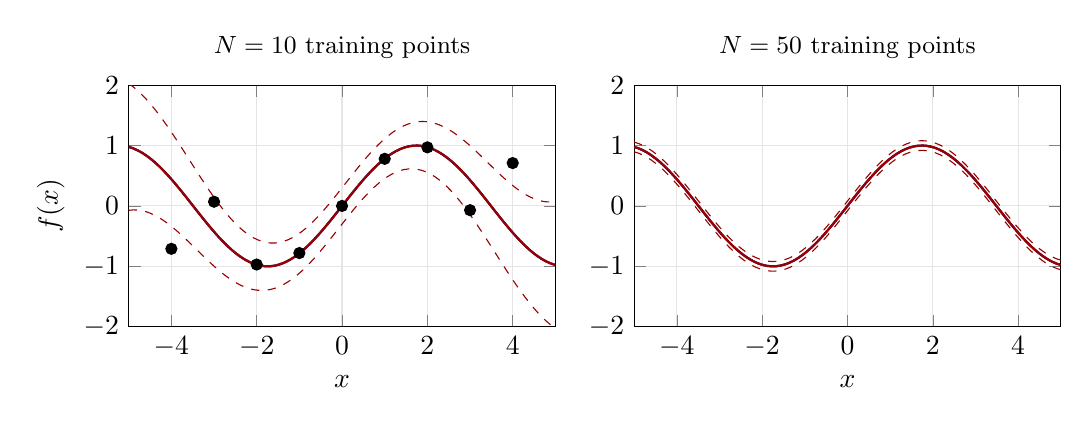
\begin{tikzpicture}
% Left panel: 10 points
\begin{axis}[
    name=left,
    width=7cm, height=4.65cm,
    title={\small $N = 10$ training points},
    xlabel={$x$}, ylabel={$f(x)$},
    xmin=-5, xmax=5, ymin=-2, ymax=2,
    grid=major, grid style={gray!20},
    every axis plot/.append style={no markers},
]
% True function
\addplot[uzhblue, thick, domain=-5:5, samples=100] {sin(deg(0.9*x))/1.0};
% Mean (same as true for good GP)
\addplot[harvardcrimson, thick, domain=-5:5, samples=100] {sin(deg(0.9*x))/1.0};
% CI upper
\addplot[harvardcrimson, thin, dashed, domain=-5:5, samples=100]
    {sin(deg(0.9*x))/1.0 + 0.3*(1 + 0.1*x^2)};
% CI lower
\addplot[harvardcrimson, thin, dashed, domain=-5:5, samples=100]
    {sin(deg(0.9*x))/1.0 - 0.3*(1 + 0.1*x^2)};
% Training points
\addplot[only marks, mark=*, mark size=2pt, black] coordinates
    {(-4,-0.71) (-3,0.07) (-2,-0.97) (-1,-0.78) (0,0)
     (1,0.78) (2,0.97) (3,-0.07) (4,0.71)};
\end{axis}

% Right panel: 50 points
\begin{axis}[
    at={(left.east)}, anchor=west, xshift=1cm,
    width=7cm, height=4.65cm,
    title={\small $N = 50$ training points},
    xlabel={$x$},
    xmin=-5, xmax=5, ymin=-2, ymax=2,
    grid=major, grid style={gray!20},
    every axis plot/.append style={no markers},
]
\addplot[uzhblue, thick, domain=-5:5, samples=100] {sin(deg(0.9*x))/1.0};
\addplot[harvardcrimson, thick, domain=-5:5, samples=100] {sin(deg(0.9*x))/1.0};
\addplot[harvardcrimson, thin, dashed, domain=-5:5, samples=100]
    {sin(deg(0.9*x))/1.0 + 0.08};
\addplot[harvardcrimson, thin, dashed, domain=-5:5, samples=100]
    {sin(deg(0.9*x))/1.0 - 0.08};
\end{axis}
\end{tikzpicture}
\end{center}

\vspace{0.05cm}
{\footnotesize \textcolor{uzhblue}{\textbf{Blue:}} true function. \textcolor{harvardcrimson}{\textbf{Red:}} posterior mean. \textcolor{harvardcrimson}{\textbf{Dashed:}} 95\% confidence interval. \\
More data $\Rightarrow$ tighter confidence intervals.}
\end{frame}

% --- Slide 30: Algorithmic Complexity ---
\begin{frame}[shrink=5]{Algorithmic Complexity}
\begin{block}{Cost of GP inference}
\begin{itemize}
  \item \textbf{Training:} Cholesky decomposition of $K_y \in \R^{N \times N}$: \emphc{$O(N^3)$}.
  \item \textbf{Prediction (per test point):} $O(N)$ for mean, $O(N^2)$ for variance.
  \item \textbf{Hyperparameter optimization:} $O(N^3)$ per gradient step.
\end{itemize}
\end{block}

\vspace{0.15cm}
\begin{block}{Scaling strategies for large $N$}
\begin{itemize}
  \item \textbf{Sparse GPs:} Inducing point methods --- approximate $K$ with rank-$M$ matrix ($M \ll N$), cost $O(NM^2)$.
  \item \textbf{Random features:} Approximate kernel with random Fourier features.
  \item \textbf{GPyTorch:} KISS-GP, structured kernel interpolation, GPU acceleration.
\end{itemize}
\end{block}

\vspace{0.1cm}
{\footnotesize For the surrogate problems in this course ($N \leq 10^4$, $d \leq 10$), standard GPs are sufficient.}
\end{frame}

% --- Slide 31: GPs vs DNNs ---
\begin{frame}{GPs vs DNNs: When to Use Which}
\begin{center}
\footnotesize
\setlength{\tabcolsep}{4pt}
\begin{tabular}{l l l}
\toprule
\textbf{Criterion} & \textbf{Gaussian Processes} & \textbf{Deep Neural Networks} \\
\midrule
Uncertainty quantification & \textcolor{darkgreen}{Built-in (posterior variance)} & \textcolor{darkred}{Requires ensembles / MC dropout} \\
Hyperparameter tuning & \textcolor{darkgreen}{Marginal likelihood} & \textcolor{softorange}{Grid search / Bayesian opt.} \\
Scaling with $N$ & \textcolor{darkred}{$O(N^3)$, limit $\sim 10^4$} & \textcolor{darkgreen}{$O(N)$ per epoch} \\
Scaling with $d$ & \textcolor{darkred}{Curse of dimensionality} & \textcolor{darkgreen}{Handles $d \gg 100$} \\
Small data ($N < 100$) & \textcolor{darkgreen}{Excellent} & \textcolor{darkred}{Typically underfits} \\
Training & \textcolor{darkgreen}{Closed-form} & \textcolor{softorange}{SGD, many epochs} \\
Interpretability & \textcolor{darkgreen}{Kernel encodes prior} & \textcolor{darkred}{Black box} \\
\bottomrule
\end{tabular}
\end{center}

\vspace{0.3cm}
\begin{alertblock}{Rule of thumb}
{\small
\begin{itemize}\itemsep0pt
  \item \textbf{$d \leq 10$, need UQ:} GPs (+ BAL).
  \item \textbf{$d > 10$, large data:} DNNs.
\end{itemize}}
\end{alertblock}
\end{frame}

% --- Slide 31b: Deep Kernel Learning ---
\begin{frame}{Deep Kernel Learning: Neural Features + GP Uncertainty}
\small
\begin{columns}[T]
\begin{column}{0.54\textwidth}
\textbf{Idea:} learn a feature map $\phi_{\theta}(\x)$ with a neural network, then use
\[
\textstyle k_{\text{DKL}}(\x,\x') = k_{\text{base}}\bigl(\phi_{\theta}(\x), \phi_{\theta}(\x')\bigr)
\]
so the GP operates in the learned feature space.

\vspace{0.05cm}
\begin{itemize}\itemsep0.1em
  \item \textbf{Front end:} the DNN learns a geometry where the target is smoother.
  \item \textbf{Back end:} the GP still provides posterior mean and variance.
  \item \textbf{Training:} optimize the feature map and kernel hyperparameters via the GP marginal likelihood.
\end{itemize}

\end{column}

\begin{column}{0.42\textwidth}
\begin{center}
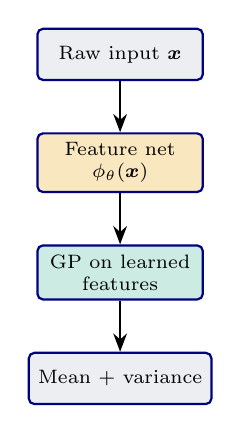
\begin{tikzpicture}[
    box/.style={rectangle, draw=uzhblue, fill=uzhgreylight, rounded corners=2pt,
        minimum width=2.1cm, minimum height=0.65cm, align=center, font=\scriptsize, thick},
    >=Stealth
]
\node[box] (raw) {Raw input $\x$};
\node[box, below=0.65cm of raw, fill=softorange!25] (net) {Feature net\\$\phi_{\theta}(\x)$};
\node[box, below=0.65cm of net, fill=softgreen!20] (gp) {GP on learned\\features};
\node[box, below=0.65cm of gp] (out) {Mean + variance};
\draw[->, thick] (raw) -- (net);
\draw[->, thick] (net) -- (gp);
\draw[->, thick] (gp) -- (out);
\end{tikzpicture}
\end{center}
\end{column}
\end{columns}
\end{frame}

% --- Slide 31c: When DKL Helps ---
\begin{frame}{When Do Deep Kernels Help?}
\begin{columns}[T]
\begin{column}{0.52\textwidth}
\textbf{Standard GP assumption:} Euclidean distance in the \emph{raw input space} is informative.

\vspace{0.2cm}
\textbf{Failure modes:}
\begin{itemize}
  \item Hidden regimes / thresholds / nonstationarity
  \item Inputs are badly warped coordinates of a simple latent state
  \item Moderate-to-high-dimensional raw features with strong correlations
  \item You still need \emphc{uncertainty quantification} or BAL
\end{itemize}
\end{column}

\begin{column}{0.43\textwidth}
\begin{alertblock}{Rule of thumb}
\begin{itemize}
  \item If the input is already low-dimensional and smooth: \textbf{plain GP} is usually enough.
  \item If the latent structure is smooth but the raw geometry is poor: \textbf{DKL} is often the right bridge.
  \item If $d$ is huge and UQ is not central: \textbf{pure DNN surrogate}.
\end{itemize}
\end{alertblock}
\end{column}
\end{columns}

\vspace{0.2cm}
{\small In short: \emphc{DKL answers the question ``Can we combine DNN feature learning with GP uncertainty?''}}
\end{frame}

% --- Slide 32: Summary Part II ---
\begin{frame}{Summary: Gaussian Process Regression}
\begin{enumerate}
  \item \textbf{GPs} = nonparametric Bayesian regression with \emphc{built-in UQ}.
  \item \textbf{Kernel} encodes prior beliefs (smoothness, scale, periodicity).
  \item \textbf{Posterior:} closed-form mean and variance, conditioned on data.
  \item \textbf{Hyperparameters:} learned by maximizing the marginal likelihood (automatic Occam's razor).
  \item \textbf{Limitation:} $O(N^3)$ scaling; best for moderate $N$ and $d$.
  \item \textbf{DKL:} neural feature extractor + GP head = useful when raw inputs are warped or moderately high-dimensional, but you still want UQ.
\end{enumerate}

\vspace{0.3cm}
\textbf{Next:} Use the GP's uncertainty to \emphc{intelligently select training points} --- Bayesian Active Learning.
\end{frame}

% ============================================================================
% PART III: BAYESIAN ACTIVE LEARNING
% ============================================================================

\end{document}
